% main.tex -- PRL-style manuscript (REVTeX 4.2). Direction 11, revised for iteration 6 (matched-EO comparison).
% ALL device numbers are SIMULATION / design predictions (sources: ../data/iter5_final.json,
% ../data/iter6_fair.json (main line), ../data/iter5_power_sweep.csv, ../data/iter5_Q_sweep.csv, ../data/key_results.json, ./eo_baseline.json).
% Literature numbers: see per-entry verification comments in refs.bib.
\documentclass[aps,prl,reprint,superscriptaddress,amsmath,amssymb,floatfix]{revtex4-2}
\usepackage{graphicx}
\usepackage{bm}
\usepackage[colorlinks=true,linkcolor=blue,citecolor=blue,urlcolor=blue]{hyperref}
\newcommand{\etash}{\eta_{\rm shift}}
\newcommand{\etaabs}{\eta_{\rm abs}}

\begin{document}

\title{Acoustically driven photonic-molecule frequency shifter on suspended thin-film lithium niobate: a simulation study of a $\sim$440-fold reduction in drive power}

\author{Xinlei Chen}
\affiliation{Affiliation to be added}
% TODO: author list / affiliations / acknowledgements to be completed by the group.

\date{\today}

\begin{abstract}
Coupled-ring (``photonic molecule'') electro-optic (EO) frequency shifters on thin-film lithium niobate (TFLN) shift $\sim$99\% of the output light, but they need $\sim$0.1~W of microwave drive. Acoustically driven lithium niobate photonic molecules have recently been demonstrated, but no shift efficiency or insertion loss has been reported for them. We simulate their use as a high-efficiency, single-output frequency shifter at microwatt drive. The design replaces the electrodes of the EO device with a suspended interdigital-transducer (IDT) acoustic resonator, which modulates one ring over 15\% of its length. We integrate the full time-domain coupled-mode equations without the rotating-wave approximation and calibrate the drive to a measured resonant acousto-optic modulator. With the measured intrinsic quality factor of the suspended platform, $Q_i\approx2.4\times10^6$, the device shifts 98.4\% of the output light by 3.33~GHz using 7.4~$\mu$W of RF power, with 57\% absolute efficiency and 2.4~dB insertion loss. An EO drive with identical optics needs 3.25~mW, so the acoustic drive uses $\approx$440$\times$ less power (430--520$\times$ across the coupling sweep). The advantage comes from the larger supermode coupling per volt and does not depend on $Q_i$. The acoustic drive also needs $\approx$13{,}000$\times$ less power than the measured EO device (96~mW). A non-suspended variant gains only $\approx$1.2$\times$ over its matched EO drive, which shows that comparing with the measured device alone overstates the acoustic benefit. The costs are a fixed shift frequency, an RF bandwidth of only $\sim$1~MHz instead of $>$3~GHz, and higher loss. The drive strength comes from extrapolating the coupling to partial ring coverage, which has not yet been verified experimentally. IDT impedance mismatch is not modeled, so the real RF power may be higher.
\end{abstract}

\maketitle

% ---------------------------------------------------------------- Introduction
\emph{Introduction.}---Encoding photonic qubits in discrete frequency bins requires low-loss, coherent devices that move photons between bins~\cite{Lukens2017,Kues2017,Lu2018}. TFLN supports such devices because it combines strong Pockels, piezoelectric, and photoelastic responses with ultralow-loss resonators~\cite{Wang2018,Zhang2017,Zhu2026loss}. Recent TFLN demonstrations include single-photon spectral shearing over $\pm641$~GHz~\cite{Zhu2022}, an integrated quantum frequency processor~\cite{Yang2026}, and coupled-cavity frequency beam splitters~\cite{Cohen2026}. The coupled-ring shifter of Hu \emph{et al.}~\cite{Hu2021} is the benchmark for single-tone shifting. A microwave drive hybridizes the symmetric (S) and antisymmetric (AS) supermodes of a photonic molecule~\cite{Zhang2019}. When the coupling rates satisfy a generalized critical-coupling condition, the light transfers in one direction between the two supermodes. The device shifts 98.7\% of the output light by 28.2~GHz with 0.45~dB insertion loss (IL), and 99.1\% (up) and 99.4\% (down) at 12.5~GHz~\cite{Hu2021}. It requires 96~mW of microwave power (3.1~V peak at the 50-$\Omega$ probe). Our literature search for 2022--2026 found no measured EO coupled-ring shifter with a lower drive power, so this device remains our measured baseline. The search was not exhaustive. A different EO approach, serrodyne driving of cascaded traveling-wave TFLN phase modulators, reports $>$98.8\% shift efficiency with $V_\pi\approx2.3$~V and broadband operation~\cite{Qiu2025}.% TODO(verify): Qiu2025 abstract only.
 For many-channel or cryogenic frequency-domain processors, this drive power sets the heat load.

Acoustic resonators on TFLN boost the microwave-to-optical phase modulation through resonance. A suspended 100-$\mu$m resonator at 3.33~GHz gives $V_\pi=4.6$~V ($V_\pi L=0.046$~V\,cm) with one arm modulated~\cite{Shao2019}. A non-suspended push-pull modulator gives $V_\pi L=1.004$~V\,cm at 0.842~GHz~\cite{Ni2026}. Acoustic waves have been used to modulate integrated resonators~\cite{Tadesse2014} and to control a photonic molecule dynamically~\cite{Kapfinger2015}. On LN-on-sapphire, Zhu \emph{et al.} recently drove a coupled-microring photonic molecule acoustically at 8.54~GHz~\cite{Zhu2025ao}. A backward-Brillouin dynamic Bragg mirror produced strong supermode coupling at $\sim$0.6~mW of acoustic power, with frequency conversion and a cooperativity of 2.46~mW$^{-1}$. That work reports no shift efficiency or insertion loss for frequency-shifter operation, so acoustic driving of a photonic molecule is not itself new. Our design differs in three ways: a co-directional, single-bus shifter, high-$Q$ supermodes, and an analysis of $\etash$, loss, and the required RF power. In a related microring, Xu \emph{et al.} measured an acousto-optic coupling $G^2=\alpha P_a$ with $\alpha=1774$~GHz$^2$/W and an RF-to-acoustic IDT efficiency of $\approx$10\%~\cite{Xu2025b}. This implies couplings of order 0.1~GHz at a few $\mu$W of acoustic power, the same order as the supermode coupling our design needs. Their geometry (a traveling 8.5-GHz wave without an acoustic cavity) differs from ours, so this result supports the plausibility of $\mu$W-scale coupling but does not calibrate our design. An optomechanical single-photon shifter with near-unity efficiency has also been demonstrated~\cite{Fan2016}. % TODO(verify): Fan2016 checked against abstract only; keep qualitative.
Traveling-wave TFLN acousto-optic shifters, however, reach only 3.5\% on-chip efficiency at 30~dBm~\cite{Shao2020}. Here we ask whether an acoustic resonator can replace the electrodes of the Hu architecture. We compare it with an EO drive of identical optical parameters as well as with the measured device. All device numbers below come from simulation; none are measurements.

% ---------------------------------------------------------------- Model
\emph{Model.}---We follow Eq.~(S2) of Ref.~\cite{Hu2021}. Two identical rings ($a_{1,2}$) couple to each other at rate $\mu$, and ring~1 couples to the bus at rate $\gamma$. Both rings have intrinsic loss $\kappa_i$. Only ring~1 lies in the acoustic field, so its resonance is modulated as $\delta\omega\cos\Omega_m t$:
\begin{align}
\dot a_1&=\Big[-i\big(\Delta+\delta\omega\cos\Omega_m t\big)-\tfrac{\gamma+\kappa_i}{2}\Big]a_1-i\mu a_2-\sqrt{\gamma}\,\alpha_{\rm in},\nonumber\\
\dot a_2&=\Big[-i\Delta-\tfrac{\kappa_i}{2}\Big]a_2-i\mu a_1,\qquad a_{\rm out}=\alpha_{\rm in}+\sqrt{\gamma}\,a_1 .
\label{eq:eom}
\end{align}
The laser is tuned to the S mode ($\Delta=\mu$), and the doublet splitting is matched to the acoustic frequency, $2\mu=\Omega_m$. We integrate Eq.~\eqref{eq:eom} with a fourth-order Runge--Kutta scheme (80 steps per period) and make no rotating-wave approximation. We then project $a_{\rm out}$, averaged over the final 20~ns, onto the frequencies $\omega_L+q\Omega_m$ ($|q|\le3$). In the S/AS basis the single-ring term becomes $\tfrac{\delta\omega}{2}\cos\Omega_m t\,(c_S^\dagger c_S+c_A^\dagger c_A+c_S^\dagger c_A+{\rm h.c.})$. The supermode coupling is therefore $\delta\omega/2$, and the critical condition becomes $\delta\omega\simeq\gamma$. We define the efficiencies as in Ref.~\cite{Hu2021}: $\etash=P_{\rm shift}/P_{\rm out}$, $\etaabs=P_{\rm shift}/P_{\rm in}$, and ${\rm IL}=-10\log_{10}(P_{\rm out}/P_{\rm in})$.

We calibrate the drive to the measured single-arm resonant MZI~\cite{Shao2019}. A peak voltage $V$ at a 50-$\Omega$ source ($P_{\rm RF}=V^2/2R$) produces the phase $\Delta\phi=\pi VL_a/(V_\pi L)$ over the covered length $L_a=100~\mu$m. This phase shifts the ring resonance by
\begin{equation}
\delta\omega=\Delta\phi\,\frac{c}{n_g L_{\rm ring}},\qquad n_g=2.3 ,
\label{eq:cal}
\end{equation}
with $L_{\rm ring}=0.667$~mm (coverage 15\%) and $\Omega_m/2\pi=3.33$~GHz. This gives $\delta\omega/2\pi=21.3$~GHz/V, i.e., a supermode coupling of 10.6~GHz/V. For the intrinsic loss we use the value implied by the suspended racetrack of the same work, $\kappa_i/2\pi=0.85\times95~{\rm MHz}=80.75$~MHz, from $\kappa/2\pi=95$~MHz and $2\kappa_e/\kappa=0.3$~\cite{Shao2019}. This corresponds to $Q_i\approx2.4\times10^6$ at 193.4~THz. The matched EO baseline uses the same equations with Hu's push-pull term $\pm\Omega\cos\Omega_m t$ on both rings. It assumes Hu's EO coefficient of $\Omega/2\pi\approx0.5$~GHz/V~\cite{Hu2021} and an electrode voltage equal to the probe voltage ($V_c=V_0$).

\begin{figure}[t]
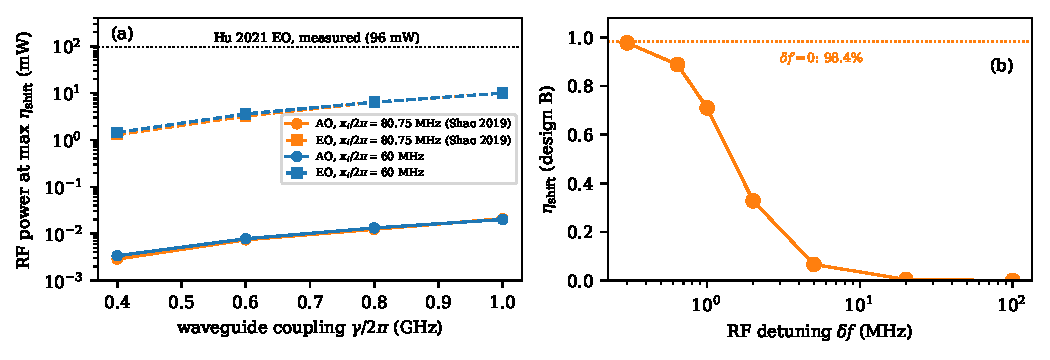
\includegraphics[width=\columnwidth]{figures/fig6_fair.pdf}
\caption{Matched comparison for the suspended design (simulation). (a)~RF power at maximum $\etash$ versus waveguide coupling $\gamma$ for the acoustic drive (circles) and the same-optics EO drive (squares). Results are shown for the Shao-measured loss $\kappa_i/2\pi=80.75$~MHz (orange) and for $\kappa_i/2\pi=60$~MHz (blue). The dotted line marks the measured 96~mW of Ref.~\cite{Hu2021}. (b)~$\etash$ versus RF detuning $\delta f$ of the drive from the doublet splitting, at $\gamma/2\pi=0.6$~GHz and $\kappa_i/2\pi=80.75$~MHz. The drive amplitude follows an acoustic Lorentzian of linewidth 1.28~MHz.}
\label{fig:fair}
\end{figure}

% ---------------------------------------------------------------- Results
\emph{Results.}---At $\gamma/2\pi=0.6$~GHz the acoustic drive reaches $\etash=98.4\%$ at $P_{\rm RF}=7.4~\mu$W (27~mV peak, $\delta\omega/2\pi=579$~MHz), with $\etaabs=57\%$ and IL $=2.4$~dB (Table~\ref{tab:main}). The same-optics EO drive needs 3.25~mW (0.57~V) for $\etash=99.7\%$, which is a factor of $\approx$440 more. Across $\gamma/2\pi=0.4$--1.0~GHz and both $\kappa_i$ values the factor stays between 430 and 520 [Fig.~\ref{fig:fair}(a)]. It is set by the ratio of supermode couplings per volt: $(10.6/0.5)^2\approx450$. Because this ratio does not involve the optical linewidth, it is essentially independent of $Q_i$. The power is also $\approx$13{,}000$\times$ below the measured 96~mW~\cite{Hu2021}. That larger factor includes the narrower linewidth ($\gamma/2\pi=0.6$ vs 5.31~GHz), which a 3.33-GHz EO molecule could equally exploit.

This comparison matters because the larger factor alone can mislead. A non-suspended design calibrated to Ref.~\cite{Ni2026} (0.842~GHz, $Q_i\approx1.9\times10^7$) needs 79~$\mu$W, which is $\approx$1{,}200$\times$ below the measured device. Its same-optics EO drive, however, needs only 95~$\mu$W, so its acoustic advantage is a mere 1.2$\times$. That advantage comes from the optical $Q$, not from the acoustics, and we do not claim it (Supplemental Material, Fig.~\ref{fig:main}).

Single-ring driving has a cost. The common-mode term phase-modulates both supermodes and creates parasitic orders. At the operating point, the largest is $q=-1$ at $-21.2$~dB relative to the shifted line ($q=+2$ at $-23.2$~dB), and the carrier is at $-24.8$~dB. Push-pull EO driving cancels this term, which is why the EO $\etash$ is slightly higher. For HOM-type interference the parasitic orders must be filtered. We did not separately simulate HOM visibility or thermal-phonon phase noise.

\begin{table}[b]
\caption{Operating points at $\gamma/2\pi=0.6$~GHz (simulation; \texttt{data/iter6\_fair.json}) compared with the measured EO shifter~\cite{Hu2021}.}
\label{tab:main}
\begin{ruledtabular}
\small
\begin{tabular}{lccc}
 & AO (sim.) & EO$^{c}$ (sim.) & Hu~\cite{Hu2021} (meas.)\\
\hline
$\Omega_m/2\pi$ (GHz) & 3.33 & 3.33 & 28.2\\
$\gamma/2\pi$ (GHz) & 0.60 & 0.60 & 5.31\\
$\kappa_i/2\pi$ (MHz) & 80.75 & 80.75 & 170\\
$Q_i$ & $2.4\times10^6$ & $2.4\times10^6$ & $1.1\times10^6$\\
Coupling (GHz/V) & 10.6 & 0.5$^{b}$ & 0.5$^{b}$\\
$\etash$ & 98.4\% & 99.7\% & 98.7\%\\
Peak voltage & 27~mV & 0.57~V & 3.1~V\\
$P_{\rm RF}$ & 7.4~$\mu$W & 3.25~mW & 96~mW\\
IL (dB) & 2.4 & 2.4 & 0.45\\
$\etaabs$ & 57\% & 57\% & $\approx$89\%\\
Max.\ spur (dB) & $-21.2$ & --- & ---\\
RF bandwidth & $\sim$1~MHz$^{a}$ & not sim. & $>$3~GHz\\
\end{tabular}
\end{ruledtabular}
\raggedright\footnotesize $^{a}$$\etash\ge97.8\%$ within $\pm0.3$~MHz, 71\% at 1~MHz, and 33\% at 2~MHz [Fig.~\ref{fig:fair}(b)]. $^{b}$S--AS supermode coupling per volt, on the electrode capacitor~\cite{Hu2021}; the baseline assumes $V_c=V_0$. $^{c}$Push-pull EO drive with the same optics.
\end{table}

\emph{Bandwidth and frequency.}---The cost of the gain is bandwidth. Detuning the drive from the doublet splitting [Fig.~\ref{fig:fair}(b)] keeps $\etash\ge97.8\%$ only within $\pm0.3$~MHz. It falls to 89\% at 0.64~MHz, 71\% at 1~MHz, and 33\% at 2~MHz. The usable RF bandwidth is therefore $\sim$1~MHz, compared with $>$3~GHz for the EO device~\cite{Hu2021}. The shift frequency is fixed at the 3.33~GHz acoustic resonance, whereas the EO device has been operated at 11--28.2~GHz~\cite{Hu2021}. The doublet splitting must also match $\Omega_m$ to well within the optical linewidth, which requires thermal tuning.

\emph{Fairness of the baseline.}---The EO baseline omits two things. First, Hu \emph{et al.} note that a microwave cavity could reduce the drive voltage~\cite{Hu2021}. An EO electrode inside an on-chip microwave resonator with loaded $Q\approx450$ could in principle close the $\approx$440$\times$ gap, also with a narrow bandwidth. To our knowledge, no such resonantly driven photonic-molecule shifter has been demonstrated. Second, setting $V_c=V_0$ favors our design. Hu's circuit model gives $V_c=1.72V_0$ at 28.2~GHz~\cite{Hu2021}, and a capacitive electrode could reduce the EO power by up to $\sim$4$\times$. Our advantage would then shrink to roughly $\sim$110$\times$. We did not model the electrode circuit at 3.33~GHz.

% ---------------------------------------------------------------- Limitations
\emph{Limitations.}---These are design predictions, subject to the following caveats.
(i)~\emph{Drive strength.} We obtain $\delta\omega$ by extrapolating the published resonant $V_\pi L$~\cite{Shao2019} linearly to a ring that the acoustic field covers only partially (15\%). The extrapolation assumes the same IDT efficiency, mode overlap, and uniform acoustic phase along the covered section as in the MZI. Because the 440$\times$ factor scales as the square of the per-volt coupling, any error in this extrapolation enters squared. The extrapolation needs experimental verification. The value $n_g=2.3$ is assumed.
(ii)~\emph{Fixed frequency, narrow bandwidth.} The RF bandwidth is $\sim$1~MHz, and the shift frequency is fixed at 3.33~GHz (see above). The detuning model uses the 1.28-MHz acoustic linewidth of the 2.007-GHz mode in Table~S2 of Ref.~\cite{Shao2019}.
(iii)~\emph{Loss.} IL is 2.4~dB versus 0.45~dB measured in Ref.~\cite{Hu2021}, so the absolute efficiency is lower (57\% vs $\approx$89\%). With $\kappa_i/2\pi=60$~MHz it would be 66\%.
(iv)~\emph{Quality factor.} The power ratio does not depend on $Q_i$, but the loss does. The partly suspended ring must keep at least the Shao-measured $Q_i\approx2.4\times10^6$. The non-suspended design's apparent advantage additionally required $Q_i\gtrsim10^7$, and it disappears in the matched comparison.
(v)~\emph{Not modeled.} We did not simulate optical loss from the IDT metal or the suspended region, acoustic heating, or the resulting thermo-optic drift. Ref.~\cite{Shao2019} observed a heating-induced red shift at mW drive; our drives are at the $\mu$W level, but we have not modeled this effect.
(vi)~\emph{IDT impedance mismatch.} The drive is referred to the measured source-voltage $V_\pi$ of Ref.~\cite{Shao2019}, so the IDT transduction efficiency of that device is implicitly included. We assume, however, that the full source voltage appears across the IDT and do not model impedance mismatch or its frequency dependence. The real RF power may therefore be higher. For comparison, Ref.~\cite{Xu2025b} reports $\approx$10\% RF-to-acoustic conversion.
(vii)~\emph{Model provenance of the supporting routes.} The phononic 90$^\circ$ hybrid of the IQ route (Supplemental Material) is our reconstruction of the group's acoustic-MZI model from its equations, since no code was available. Its parameters are borrowed from GaN-on-sapphire~\cite{Xu2025}. The main result does not depend on this model.

\emph{Routes not pursued.}---We also simulated three other acoustic routes (Supplemental Material), and none outperforms published devices. An IQ single-sideband shifter is limited by the Bessel function to 33.9\%. A phase-matched intermodal shifter would need $\sim$70~W at the calibration of Ref.~\cite{Shao2020}. Cavity microwave-to-optical designs fall short of cryogenic demonstrations~\cite{Weaver2024,Jiang2023,Warner2025,Mirhosseini2020}.

\emph{Conclusion.}---In simulation, driving a TFLN photonic-molecule shifter with a suspended acoustic resonator shifts 98.4\% of the output light using 7.4~$\mu$W. At identical optics this is $\approx$440$\times$ less RF power than an EO drive, and the factor follows from the per-volt coupling, not from $Q_i$. In exchange, the shifter has a fixed frequency, a $\sim$1~MHz bandwidth, and 2.4~dB loss, and EO driving through a microwave resonator remains an undemonstrated alternative. The decisive experiment is a measurement of the acousto-optic coupling of a partially covered high-$Q$ ring, together with the loss and heating added by the IDT.

\bibliography{refs}

% ================================================================ Supplement
\clearpage
\onecolumngrid
\begin{center}\textbf{\large Supplemental Material}\end{center}
\setcounter{figure}{0}\renewcommand{\thefigure}{S\arabic{figure}}
\setcounter{table}{0}\renewcommand{\thetable}{S\arabic{table}}
\setcounter{equation}{0}\renewcommand{\theequation}{S\arabic{equation}}

The routes below are supporting material. None of them beats published results; they explain why the main text uses the resonant photonic molecule. All numbers come from simulation (\texttt{data/key\_results.json}, \texttt{data/iter5\_*}, \texttt{data/iter6\_fair.json}).

\emph{S0. Iteration-5 sweeps and the non-suspended design.} Figure~\ref{fig:main} shows the iteration-5 sweeps. In these sweeps design~B uses $\kappa_i/2\pi=60$~MHz and reaches $\etash=98.4\%$ at 7.2~$\mu$W with IL $=1.8$~dB; the main text uses the Shao-measured loss instead. Design~A (non-suspended, calibrated with Ref.~\cite{Ni2026} converted to single-arm, 2.008~V\,cm; 400~$\mu$m of a 1.2~mm ring; $\gamma/2\pi=0.10$~GHz; $\kappa_i/2\pi=10$~MHz) reaches 99.2\% at 79~$\mu$W with IL $=1.8$~dB. Its same-optics EO drive needs 95~$\mu$W (S5), so we do not claim an acoustic advantage for A. Panel~(c) shows that A works only for $Q_i\gtrsim10^7$. At $Q_i=6.4\times10^7$, $1.9\times10^7$, $6.4\times10^6$, and $1.9\times10^6$ we find $\etash=99.5$, 99.5, 98.7, and 42\%, and $\etaabs=86$, 60, 36, and 10\%.

\begin{figure*}[h]
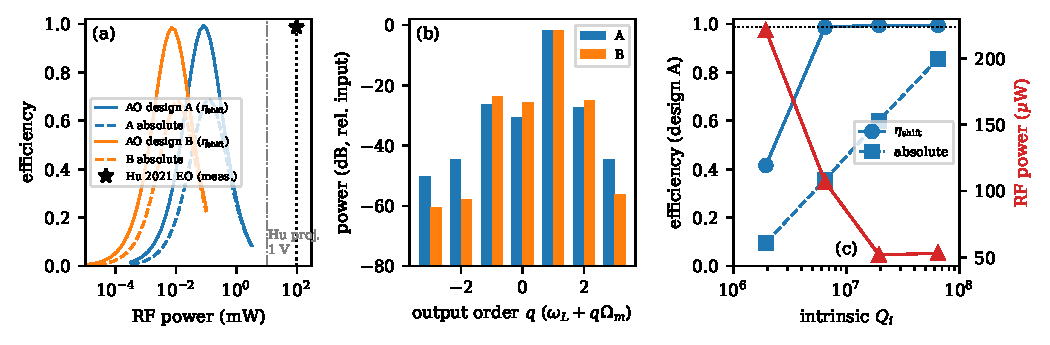
\includegraphics[width=\textwidth]{figures/fig5_ao_molecule.pdf}
\caption{Iteration-5 sweeps (simulation). (a)~$\etash$ (solid) and $\etaabs$ (dashed) versus RF power for design~A (blue, 0.842~GHz, non-suspended) and design~B (orange, 3.33~GHz, suspended, $\kappa_i/2\pi=60$~MHz). The star marks Ref.~\cite{Hu2021} (98.7\%, 96~mW). The dash-dotted line marks the authors' projected 1~V drive. (b)~Output power in each order $q$, relative to the input, at the optimum. (c)~Design~A versus $Q_i$, with $\gamma$ and $\delta\omega$ re-optimized at each point. The right axis gives the RF power.}
\label{fig:main}
\end{figure*}

\emph{S1. Acoustic IQ single-sideband shifter.} We used a 50:50 acoustic directional coupler as a phononic 90$^\circ$ hybrid; its two output ports differ by $-90.0^\circ$, as verified numerically. The two outputs drive the I and Q push-pull sub-MZIs of a nested optical IQ modulator. The model is reconstructed from equations, with GaN parameters~\cite{Xu2025}: coupler full-transfer length 79.14~$\mu$m, thermo-acoustic phase 4.03~rad/W, and 2.4~dB/mm acoustic loss. The reconstructed DC--arm--DC model reproduces $T=\tfrac12[1+\cos(\alpha P_H+\phi_0)]$ to within $4\times10^{-16}$. The ideal shifted-sideband power is $J_1^2(\Delta\phi/2)$, with a maximum of 33.9\% at $\Delta\phi=3.68$~rad (unfiltered HOM visibility 0.969). Requiring a visibility of 0.99 lowers the efficiency to 30.1\%. With the calibration of Ref.~\cite{Ni2026}, maximum efficiency needs 19.3~W at $L=400~\mu$m or 0.77~W at $L=2$~mm (Fig.~\ref{fig:s1}). The measured EO photonic molecule reaches 98.7--99.4\%~\cite{Hu2021}.

\begin{figure}[h]
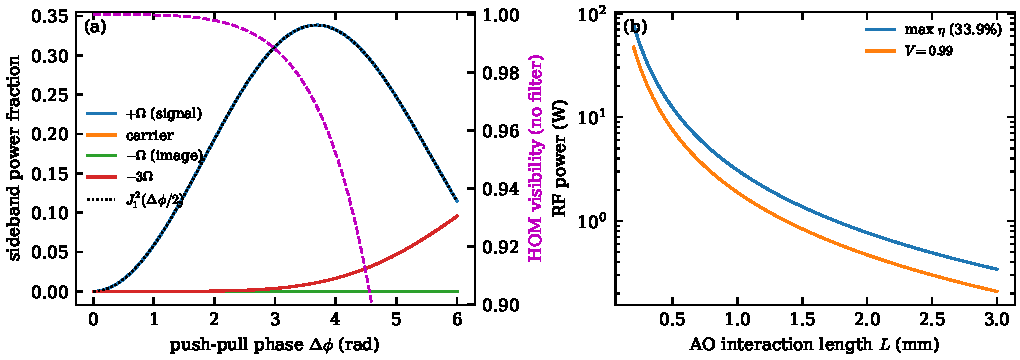
\includegraphics[width=0.75\textwidth]{figures/fig1_ssb_iq.pdf}
\caption{IQ single-sideband route. (a)~Sideband powers and unfiltered HOM visibility versus push-pull phase. (b)~Required RF power versus acousto-optic interaction length.}
\label{fig:s1}
\end{figure}

\emph{S2. Fabrication tolerance.} We ran Monte Carlo simulations (300 samples per point) of the coupler length error $\sigma_L/L$, with 0.05~rad thermal phase noise, 30~dB sub-MZI extinction, and filtering of $|n|\ge3$ orders. Without trimming, the image rejection falls from 36 to 29~dB as $\sigma_L/L$ increases from 0 to 10\%. After thermo-acoustic trimming it is 38~dB ($V=0.9997$) at 5\% and 33~dB ($V=0.9993$) at 10\%. Carrier suppression saturates near 39~dB, a limit set by the sub-MZI extinction (Fig.~\ref{fig:s2}).

\begin{figure}[h]
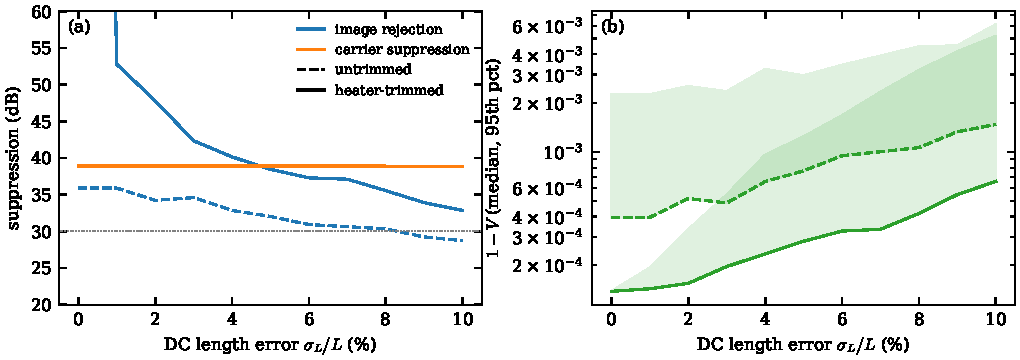
\includegraphics[width=0.75\textwidth]{figures/fig2_tolerance.pdf}
\caption{Tolerance of the IQ route to coupler length errors. (a)~Image and carrier suppression, untrimmed and heater-trimmed. (b)~HOM infidelity $1-V$.}
\label{fig:s2}
\end{figure}

\emph{S3. Phase-matched intermodal shifter.} We modeled TE$_0(\omega)\to$TE$_1(\omega+\Omega)$ conversion with coupled-mode equations, calibrated to the 3.5\% efficiency at 30~dBm of Ref.~\cite{Shao2020}. Complete lossless conversion would need about 70~W. Acoustic loss of 1--2.4~dB/mm lowers the achievable efficiency further (Fig.~\ref{fig:s3}).

\begin{figure}[h]
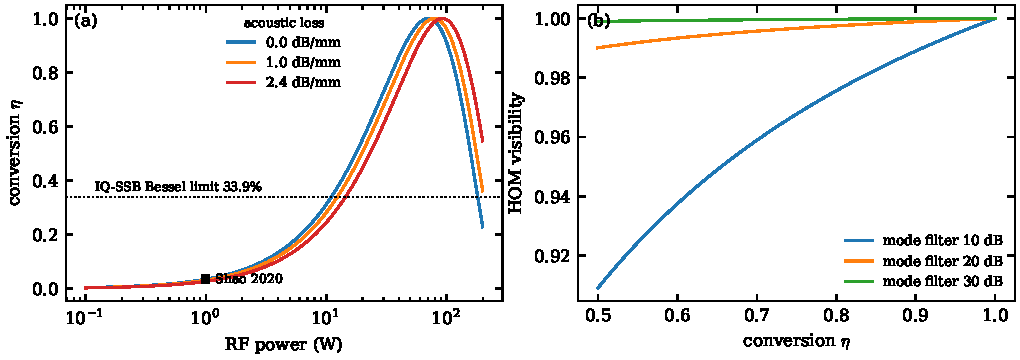
\includegraphics[width=0.75\textwidth]{figures/fig3_intermodal.pdf}
\caption{Intermodal route. (a)~Conversion efficiency versus RF power for several acoustic losses. (b)~HOM visibility versus conversion efficiency for different mode-filter extinctions.}
\label{fig:s3}
\end{figure}

\emph{S4. Microwave-to-optical conversion.} The linearized model of Ref.~\cite{Shao2019} with its Table~S2 parameters reproduces the published single-photon cooperativity, $C_0=3.98\times10^{-8}$ ($4\times10^{-8}$ published), and efficiency, $\eta=1.78\times10^{-5}$ at 1~mW (0.0017\% published). We then considered three hypothetical designs. Double resonance gives 1.8\% at 1~mW. Critically coupled optics and IDT give 25\%. Overcoupled optics and IDT ($\kappa_e/\kappa=\gamma_e/\gamma=0.9$) give 74\% at 1~mW, with a maximum of 81\%. The added noise of the overcoupled design is 346 quanta at 300~K and 0.069 at 0.1~K. This room-temperature model does not compete with cryogenic demonstrations~\cite{Weaver2024,Jiang2023,Warner2025,Mirhosseini2020} (Fig.~\ref{fig:s4}).

\begin{figure}[h]
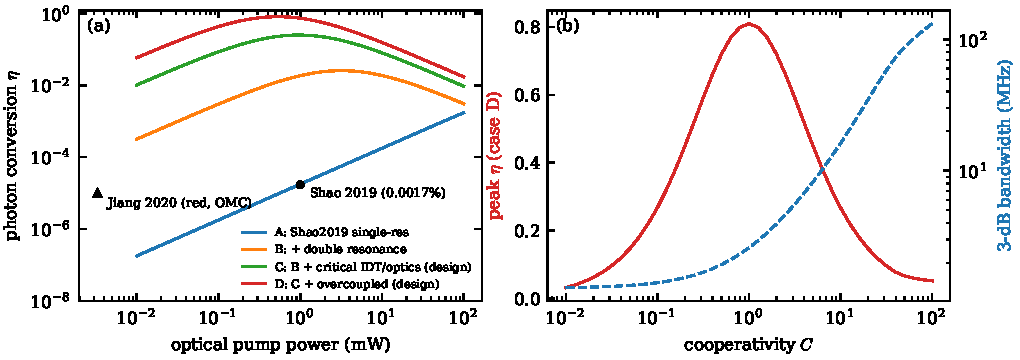
\includegraphics[width=0.75\textwidth]{figures/fig4_transducer.pdf}
\caption{Microwave-to-optical route. (a)~Photon conversion efficiency versus optical pump power. (b)~Peak efficiency and bandwidth versus cooperativity for the overcoupled design.}
\label{fig:s4}
\end{figure}

\emph{S5. Matched EO baseline} (\texttt{paper/eo\_baseline.py}; iteration-6 sweep in \texttt{iter6\_fair.py}). The baseline uses Eq.~(S2) of Ref.~\cite{Hu2021} with push-pull modulation $\pm\Omega\cos\Omega_m t$ on both rings, Hu's coefficient of $\sim$0.5~GHz/V on the capacitor~\cite{Hu2021}, the source voltage applied directly to the electrode, and $P=V^2/(2\cdot50~\Omega)$. Design~A's optics give $\Omega/2\pi=49$~MHz, $V=97.5$~mV, $\approx95~\mu$W, and $\etash=99.8\%$. Design~B's iteration-5 optics ($\kappa_i/2\pi=60$~MHz) give $\Omega/2\pi=292$~MHz, $V=0.585$~V, $\approx3.4$~mW, and $\etash=99.8\%$. In the iteration-6 sweep with $\gamma/2\pi=0.4$, 0.6, 0.8, and 1.0~GHz, the EO/AO power ratio is 427, 461, 483, and 496 at $\kappa_i/2\pi=60$~MHz. At $\kappa_i/2\pi=80.75$~MHz it is 450, 438, 516, and 478. Over the same range, the acoustic $\etash$ falls from 99.3\% to 96.0\%. Push-pull driving cancels the common-mode term, which explains the higher $\etash$.

\begin{table}[h]
\caption{Selected literature benchmarks and how each was verified.}
\begin{ruledtabular}
\begin{tabular}{p{4.2cm}p{6.6cm}p{5.4cm}}
Work & Reported metric (measured) & Verification\\
\hline
Hu \emph{et al.}~\cite{Hu2021} & 98.7\%, 0.45~dB, 96~mW @28.2~GHz; 99.1/99.4\% @12.5~GHz & arXiv full text + Supplement\\
Shao \emph{et al.} 2019~\cite{Shao2019} & $V_\pi=4.6$~V (100~$\mu$m), 3.33~GHz, $\sim$1~MHz & arXiv full text\\
Ni \emph{et al.}~\cite{Ni2026} & $V_\pi L=1.004$~V\,cm, 0.842~GHz, 132.5~MHz & arXiv abstract\\
Shao \emph{et al.} 2020~\cite{Shao2020} & 3.5\% @30~dBm, $>$30~dB carrier supp., 70~MHz & arXiv full text\\
Fan \emph{et al.}~\cite{Fan2016} & near-unity efficiency, up to 150~GHz (qualitative) & abstract only (TODO: full text)\\
Zhu \emph{et al.}~\cite{Zhu2022} & $\pm641$~GHz shearing of single photons & abstract\\
Weaver \emph{et al.}~\cite{Weaver2024} & 0.9\%, 14.8~MHz & abstract\\
Jiang \emph{et al.}~\cite{Jiang2023} & 5\% continuous conversion & abstract\\
Warner \emph{et al.}~\cite{Warner2025} & up to 1.18\% & abstract\\
\end{tabular}
\end{ruledtabular}
\end{table}

\end{document}
